\begin{figure}[htb]
    \begin{subfigure}{0.45\textwidth}
         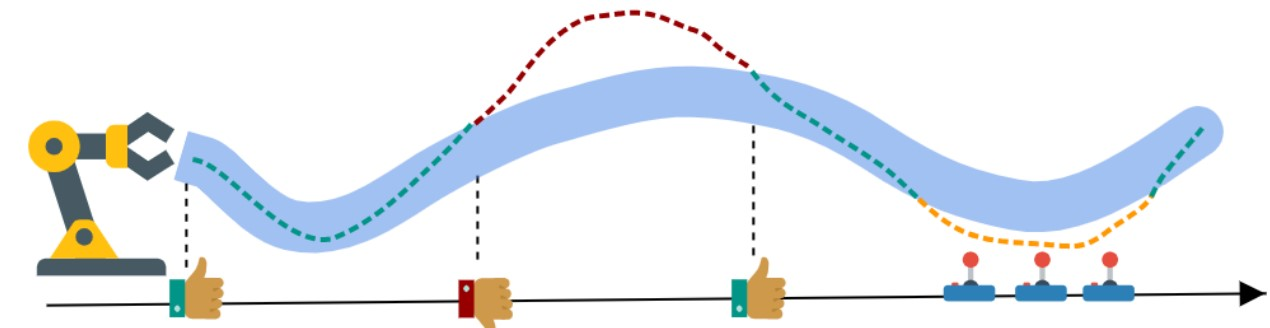
\includegraphics[width=\textwidth]{Figures/images/correct-me-if-i-am-wrong/feedback.jpg}
         \caption{Evaluative feedback: the expert labels the sub-trajectory as satisfactory or not. Corrective feedback: the human guides the robot towards the correct trajectory}
         \label{fig:feedback}
    \end{subfigure}
    \hfill
    \begin{subfigure}{0.50\textwidth}
         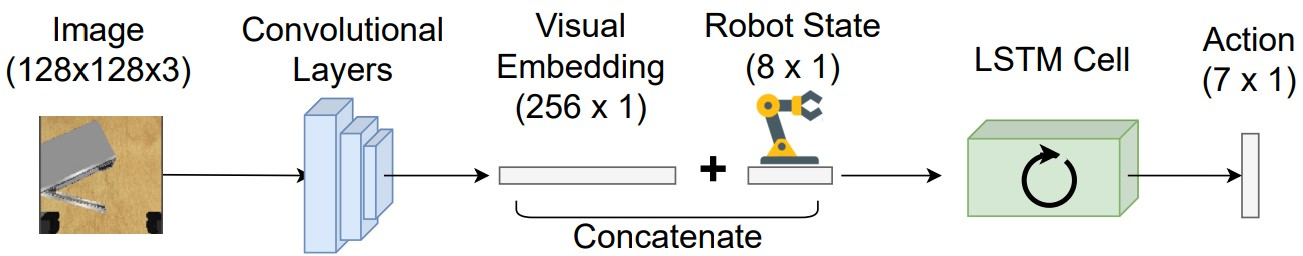
\includegraphics[width=\textwidth]{Figures/images/correct-me-if-i-am-wrong/correct_me_architecture.jpg}
         \caption{Policy architecture: The input is an RGB image of the scene, the output is the desired end-effector pose and the gripper state}
         \vspace{0.5cm}
         \label{fig:architecture}
    \end{subfigure}
    \caption{(\ref{fig:feedback}) Representation of the meaning of the feedback, (\ref{fig:architecture}) Policy architecture proposed in \cite{chisari2022correct}}
    \label{fig:correct_me_if_im_wrong}
\end{figure}
